\documentclass[12pt]{article}
\usepackage{graphicx}
\usepackage[a4paper, left = 2cm, right = 2cm, top = 2cm, bottom = 2cm]{geometry}
\usepackage{listings}
\usepackage{amssymb}
\usepackage{pgfplots} 
\usepackage{amsmath}
\usepackage{hyperref}
\usepackage{url}
\usepackage{subfig}
\usepackage{algorithm}
\usepackage{algpseudocode}
\usepackage{centernot}

\newtheorem{definition}{Definition}
\newtheorem{example}{Exmaple}
\newtheorem{property}{Property}
\newtheorem{proof}{Proof}
\newcommand{\norm}[1]{\lVert#1\rVert}
\newcommand{\abs}[1]{\lvert#1\rvert}

\begin{document}
	
	\begin{titlepage}
		
		\title{Project of Distributed Systems: Paradigms and Models \\
		Parallel Iterative Jacobi Method}
		\author{Student: Diego Arcelli\\ Student ID: 647979 \\
			Professor: Marco  Danelutto}
		\date{Academic Year 2021-2022}
		\maketitle
		\centering
		
\includegraphics[width=10cm]{./images/unipi_logo.png}
		
	\end{titlepage}
	
	\tableofcontents
	\newpage
	
	\section{Analysis of the problem}
	Notation premise: with $x_i^{(k)}$ we indicate the $i$-th entry of vector $x$ at iteration $k$. The pseudo-code to execute the Jacobi method sequentially, for a fixed amount of iterations, is shown in \ref{alg:seq}. Note that we are forced to use an auxiliary vector $x^\prime$ to compute the updated elements of $x$ for the current iteration, and then, before starting the following iteration, we copy the elements of $x^\prime$ in $x$. This is necessary because if at iteration $k$, we compute $x^{(k)}_1$ modifying $x$ in-place, then when we'll compute $x^{(k+1)}_2$, instead of using $x^{(k)}_1$, we'll use $x^{(k+1)}_1$.\\
	The algorithm is composed by three nested loops, where the first iterates $limit$ times, and the other two iterate $n$ times, so the time complexity is $O(limit\cdot n^2)$. The $swap$ function used to copy the elements of $x^\prime$ in $x$, can be implemented in $O(1)$ time complexity, by swapping the pointers of the two arrays.
	\begin{algorithm}[H]
		\caption{Sequential code for Jacobi method}\label{alg:seq}
		\begin{algorithmic}[1]
			\Require $A$ strictly diagonal dominant matrix, $b$ vector, $limit$ positive integer
			\For{$k \gets 1$ to $limit$}
			\For{$i \gets 1 $ to $n$}
			\State{$val \gets 0$}
			\For{$j \gets 1 $ to $n$}
			\If{$j \ne i$}
			\State{$val \gets val + A[i,j]* x[j]$}
			\EndIf
			\EndFor
			\State{$x^\prime[i] \gets \frac{1}{A[i,i]}(b[i]-val)$}
			\EndFor
			\State{swap($x$, $x^\prime$)}
			\EndFor
		\end{algorithmic}
	\end{algorithm}
	\noindent Let's now analyze how we can exploit the properties of the algorithm in order to parallelize it. The first important thing we notice is that in order to compute the updated values for the vector $x$ at iteration $k$, we need the full updated vector $x$ at iteration $k-1$, therefore the iterations of the algorithm need to be strictly sequential.\\
	A relevant property of the algorithm that we can notice from the pseudo-code, is that each element $x_i^{(k)}$ is computed independently from the others elements of the vector $x^{(k)}$, since to compute $x_i^{(k)}$ we just need the old vector $x^{(k-1)}$ and the matrix $A$. Therefore the iterations¸ of the loop at line 2 of the pseudo-code, can be executed in parallel, which is the classical application of a map pattern. So, if we have $nw$ workers available, we can assign to each worker a partition of indices of $x$ to compute.\\
	The innermost loop at line 4 is used to compute a sum of $n-1$ elements, which is the classical application of a reduce pattern. This is done inside the loop that we already said we can parallelize using a map pattern, so, if we want to implement also the reduce, for each one of the $nw$ workers of the map, we have to arrange other $nw^\prime$ additional workers that can be used to compute in parallel the summation.\\
	The introduction of a reduce inside each map would increase the overhead, since each worker assigned to the map would have to coordinate its computations with the workers that it uses for the reduce. Moreover, if the additional $nw\cdot nw^\prime$ workers arranged for the reduce, are just used to increase the parallel degree of the map, we would obtain the same theoretical speedup (this is shown in the time analysis section) but which much less overhead. Therefore there is no advantage in implementing the reduce.\\
	Even if we only implement the map, there some synchronization problems that we need to care about:
	\begin{enumerate}
		\item Start iteration $k+1$ only after all the workers finished their computations for iteration $k$, since the iterations must be strictly sequential 
		\item Executing the swap of the main and auxiliary vectors only after all the workers finished their computations for the current iteration, otherwise it might happen that the vectors are swapped while some workers are still computing their portion of $x^{(k)}$
		\item Keep track of the number of iterations so that all the workers will stop after $limit$ iterations
	\end{enumerate}
	The first problem can be solved simply by putting a barrier after the execution of the map, so that all the worker will be forced to wait the others before starting the next iteration. In this way we can also solve the third problem by selecting one of the worker to count the number of iterations of the algorithm executed so far. The designated worker can simply use a shared variable among the workers, that it will increase by one before the barrier. Since the variable is modified by just one worker it doesn't need synchronization mechanism to be accessed even if it is shared. This solution guarantees that before starting iteration $k$ the shared variable will have value $k$ for all the workers, so that every worker can individually check if $k = limit$ and stop its execution if it is the case. To solve the second problem we need to introduce a second barrier, which has to be placed between the end of the map an the previously defined next iteration barrier. Between this new defined barrier and the next iteration barrier, one of the workers will be selected to execute the swap (it can be the same one that counts the iterations). In this way the swap will happen only after every worker finished its computations for the current iteration and before starting the next iteration.\\
	The pseudo-code of the routine executed by a worker is showed in \ref{alg:par}.
	\begin{algorithm}[H]
		\caption{Worker pseudo-code}\label{alg:par}
		\begin{algorithmic}[1]
			\Require $A$ strictly diagonal dominant matrix, $b$ vector, $limit$ positive integer
			\While{$k < limit$}
			\For{$i \gets start $ to $end$}
			\State{$val \gets 0$}
			\For{$j \gets 1 $ to $n$}
			\If{$j \ne i$}
			\State{$val \gets val + A[i,j]* x[j]$}
			\EndIf
			\EndFor
			\State{$x^\prime[i] \gets \frac{1}{A[i,i]}(b[i]-val)$}
			\EndFor
			\State{\textbf{Vectors swap barrier}}
			\If{start = 0}
			\State{swap($x$, $x^\prime$)}
			\State{$k \gets k+1$}
			\EndIf
			\State{\textbf{Next iteration barrier}}
			\EndWhile
		\end{algorithmic}
	\end{algorithm}
	\noindent The variables $start$ and $end$ represent respectively the first and the last index of $x$ assigned to the worker. The worker that will update the iterations counter and execute the swap of the vector is the one assigned to the leftmost chunk (the one with $start = 0$). Note that both of the barriers are needed because if we only use the copy barrier, it could happen that one of the workers might start the next iteration before the designated worker could swap the vectors and update the iteration counter, so both barriers are needed. 
	
	
	\section{Time analysis}
	In the sequential case, the time required to execute the algorithm is:
	\[ T_{seq} = T_{init} + k\Big(n^2T_\oplus + T_{swap}\Big) \]
	where $k$ is the number of iterations, $n$ is the number of rows and columns of the matrix, $T_{init}$ is the time required to initialize the computations, $T_\oplus$ is the time required to compute the expression at line 6 of \ref{alg:seq} and $T_{swap}$ is the time required to perform the swap of the vectors. $T_{init}$ includes the declaration of some variable and the creation of the auxiliary array, an operation whose cost depends by $n$. If we consider negligible the initialization and the swap times, then the execution time is more or less: 
	\[ T_{seq} \approx kn^2T_\oplus \]
	In the parallel case, the loop at line 2 of \ref{alg:seq} is parallelized, so, with $nw$ workers available, the program will execute at the same time $nw$ parallel loops, each of which will iterate more or less $\frac{n}{nw}$ times. The overhead introduced is given by the forking and joining of the threads, by the time required to compute and assign tasks to the workers and by the time required to manage the barrier, so overall we have that the parallel time is:
	\[T_{par}(nw) = T_{init} + T_{split} + T_{fork} + k\Big(\frac{n}{nw}nT_\oplus + T_{synch} + T_{swap} + T_{synch}\Big) + T_{join} \]
	where $T_{fork}$ and $T_{join}$ are the times for the fork-join mechanism, $T_{split}$ is the time required to compute and split the tasks among the workers and $T_{synch}$ is the time required to handle the barrier. Again, if we consider negligible the times required for the preparations, the synchronization and the swap, then the parallel time is approximately:
	\[T_{par}(n) \approx k\frac{n}{nw}nT_\oplus \]
	If we had decided to implement the reduce too, assigning $nw_1$ workers to the map and $nw_2$ workers to each worker of the map for the reduce, then the parallel time would have changed as follows:
	\[ T^\prime_{par}(nw) \approx k\Big[\frac{n}{nw_1}\Big(\frac{n}{nw_2}T_\oplus + nw_2T_\oplus \Big) \Big] = k\frac{n}{nw_1}\frac{n}{nw_2}T_\oplus + knw_2T_\oplus \approx k\frac{n}{nw_1}\frac{n}{nw_2}T_\oplus \]
	since for each map we could have computed in parallel $nw_2$ partial sums of $\frac{n}{nw_2}$ elements each, and then we would have computed the final sum summing up the $nw_2$ partial sums. If in $T_{par}$ we set $nw = nw_1\cdot nw_2$, then the time is the same of $T^\prime_{par}$. Actually if we don't exclude from $T^\prime_{par}$ the time needed to compute the partial sums, we also have the term $k nw_2T_\oplus$, and so $T_{par}$ is even better than $T^\prime_{par}$. From this analysis we draw the conclusion that if we only implement the map, with the same resources we get an even better theoretical execution time than implementing both the map and the reduce. Furthermore the implementations of the reduce would introduce overheads and more synchronization problems that are not present if we only implement the map.\\
	The speedup we can achieve is:
	\[ Speedup(nw) = \frac{T_{init} + k\Big(n^2T_\oplus + T_{swap}\Big)}{T_{init} + T_{split} + T_{fork} + k\Big(\frac{n}{nw}nT_\oplus + T_{synch} + T_{swap} + T_{synch}\Big) + T_{join}}\]
	If we exclude the negligible times then we get:
	\[ Speedup(nw) \approx \frac{kn^2t_\oplus}{k\frac{n}{nw}nt_\oplus} = nw\]
	which is the ideal speedup which we can theoretically obtain with a map pattern. Of course to have a better estimate of the speedup we should consider the serial fraction of the program. We can make a rough estimation by considering that the total number of operations done by the algorithm is more or less in the order of $kn^2$. since we have to do some fixed amount of operations inside the three loops. Ideally, With $n$ workers, every worker could compute its own $x_i^{(k)}$ in more or less $n$ operations, reducing the number of operations to $kn$. Therefore a rough estimation of the serial fraction is:
	\[ f = \frac{kn}{kn^2} = \frac{1}{n}\]
	if we now consider the speedup given by the Amdahl's law, we have that in the best case the maximum speedup is:
	\[ Speedup < \frac{1}{f} = \frac{1}{\frac{1}{n}} = n\]
	So the speedup is upper-bounded by the number of rows/columns of the matrix. This makes sense, since in an ideal scenario, we would have a worker for each component of the vector $x$, reducing the cost of a single iteration of the algorithm from $O(n^2)$ to $O(n)$. So we should expect a better speedup as $n$ increases. 
	
	\section{Implementation details}
	The parallel program has been implemented in three versions:
	\begin{itemize}
		\item[--] The first using C++ threads 
		\item[--] The second using FastFlow
		\item[--] The third using OpenMP
	\end{itemize}
	The program has been implemented defining a class called \verb|Jacobi| which has as attributes the coefficients matrix $A$, the vector of known terms $b$ and an integer $n$ that is the size of $A$ and $b$. For each implementation of the algorithm (the sequential and the three parallel ones) there's a corresponding method to solve the linear system $Ax = b$, using that specific implementation, by providing as parameters the number of iterations of the algorithm and the number of workers (for the parallel versions). For all the implementations the solution vector $x$ is initialized setting all the elements to 0, and to assure that algorithm will converge, $A$ it's generated randomly to be strictly diagonal dominant. 
	
	\subsection{C++ threads}
	In the implementation with C++ threads I used the fork-join mechanism to spawn $nw$ threads, each of them is assigned to a contiguous chunk of $x$ of size $\lfloor\frac{n}{nw}\rfloor$ according to the following procedure:
	\begin{algorithmic}
		\State $\Delta \gets \lfloor\frac{n}{nw}\rfloor$
		\For{$i \gets 0$ to  $nw$}
			\State $start_i \gets i*\Delta$
			\State $end_i \gets start_i + \Delta - 1$
		\EndFor
		\State $end_{nw} \gets n-1$
	\end{algorithmic}
	Then each thread will execute code identical to the one in \ref{alg:par}. For the implementation of the barrier I used the \verb*|barrier| class introduced in C++20.
	\subsection{FastFlow}
	For the FastFlow implementation I used the \verb|ParalleFor| class to parallelize the loop at line 2 of \ref{alg:seq}. An object of class \verb|ParalleFor| is created before the loops start, in order to prepare the $nw$ workers in advance, and then we call the \verb*|parallel_for| method, inside the main loop of of the algorithm. The function passed to the parallel:
	\begin{algorithmic}
		\Function{parallel\_for\_iteration}{$i$}
		\State $val \gets 0$
		\For{$j \gets 0$ to  $n-1$}
		\If{$i \ne j$}
		\State $val \gets val + A[i,j]$
		\EndIf
		\EndFor
		\State $x^\prime[i] = (b[i]-val)/A[i,i]$
		\EndFunction
	\end{algorithmic}
	After the call of the parallel for method, the counter of the loop is increased and the vectors are swapped, and this is done sequentially by the main thread of the program. Note that we do not need to explicitly define the barrier since the call of the \verb*|parallel_for| method is an implicit barrier for the workers. 
	\subsection{OpenMP}
	For the OpenMP implementation I simply parallelized the second innermost loop at line 2 of algorithm \ref{alg:seq}, using the \verb|#pragama omp paralle for| directive, with the default static scheduling, which divides the loop in $nw$ chunks of equal size. Like in the case of FastFlow, the end of the parallelized for is an implicit barrier for the threads used in the parallel for, so we do not need to define the barrier explicitly.  
	\section{Manual}
	The source code, the scripts written for the experiments and a detailed manual of the program are available at \href{https://github.com/DiegoArcelli/Parallel-And-Distributed-Systems-Project}{this} repository.\\ 
	To compile the code is sufficient to execute the command \verb*|make| in the \verb*|src| directory of the project. The compilation will produce the executable \verb*|main| which can be launched to execute the program, providing the following arguments:
	\begin{itemize}
		\item[--] \verb|n|: the number of row and columns of the matrix
		\item[--] \verb|nw|: the number of workers that will be used in the parallel versions of the algorithm
		\item[--] \verb|iters|: the number of iterations of the algorithm
		\item[--] \verb|mode|: an integer number which specifies which implementations of the algorithm will be executed
	\end{itemize} 
	The possible values of \verb|mode|, with the corresponding effects, can be showed by launching the program with no argument. Once executed the program will run the versions of the algorithm required (according to the value of \verb|mode|), and it will print their execution times. 
	
	\section{Experiments}
	The main goals of the experiments that we will execute are the following: 
	\begin{itemize}
		\item[--] Comparing the performances obtained by the three implementations 
		\item[--] Check how the performances change with respect to the size of the matrix
		\item[--] Comparing the actual performances to the ideal ones
	\end{itemize}
	To compare the performances of the three implementations we'll measure the times obtained when executing the algorithm with $nw$ workers, varying $nw$ from 1 to 128. Then from the times we'll derive the speedup and the efficiency of the three implementations. To see if the size of the matrix impact on the performances, we'll repeat this procedure twice, first on 1000$\times$1000 matrix and then on a 1000$\times$1000 matrix.\\
	After that we'll select the number of workers for which we obtain the best speedup and we'll execute the algorithms with that number of workers for matrices of different sizes (500, 1000, 5000, 10000, 15000, 20000) to better understand the impact that the size of the matrix has on the performances.\\
	Another interesting fact that I encountered during the experiments and I think it's worth mentioning, is  that the data type of the elements of the matrix has a significant impact on the achieved speedup of the parallel implementations. Using \verb|floats| data type yields to better speedups than using \verb|double| or \verb|long double|. Because of this I also inserted a plot that shows the different speedup achieved by the FastFlow implementation for the three C++ floating point data type \verb|float|, \verb|double| and \verb|long double|. \\
	To get the times I created a \verb|timer| class which uses the RAII mechanism to print the difference between the time in which it's created and the time in which it's destructed, as we saw during the lectures. In the execution time are included the declaration of some variable and the allocation and deallocation of the auxiliary array in the main memory, but not the initialization of vector $x$.\\
	The results of the experiments are shown in the below plots:
	
	\begin{figure}[H]
		\centering
		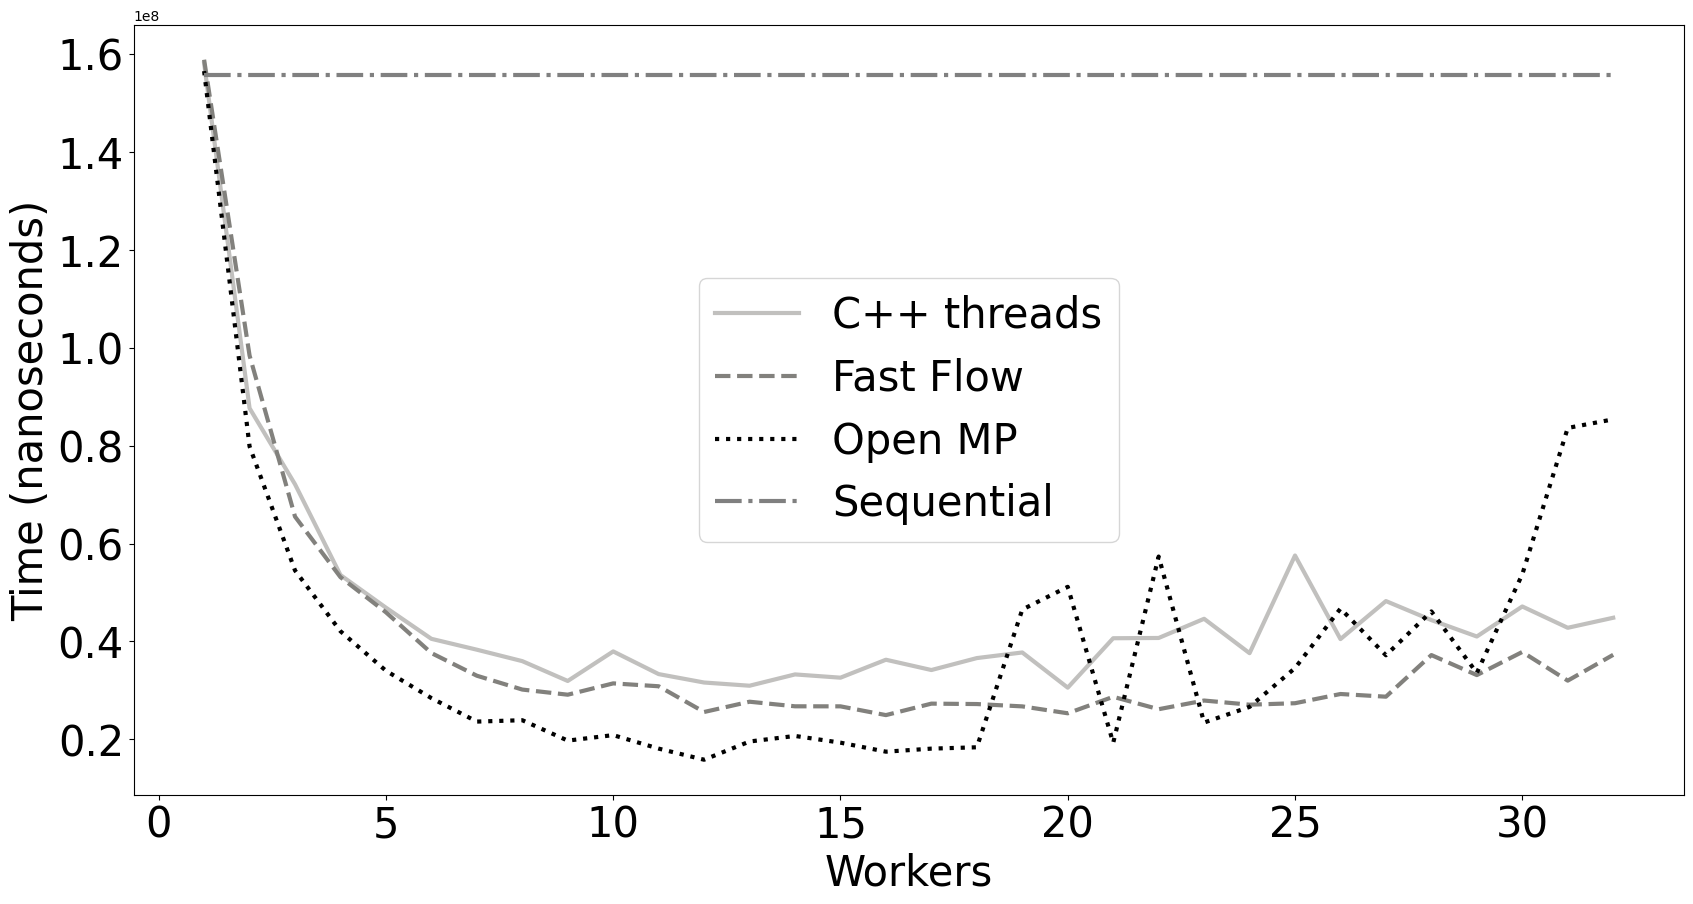
\includegraphics[width=13cm]{./images/time_vs_cores_1000}
		\caption{Time vs workers for matrix size 1000}
	\end{figure}
	
	\begin{figure}[H]
		\centering
		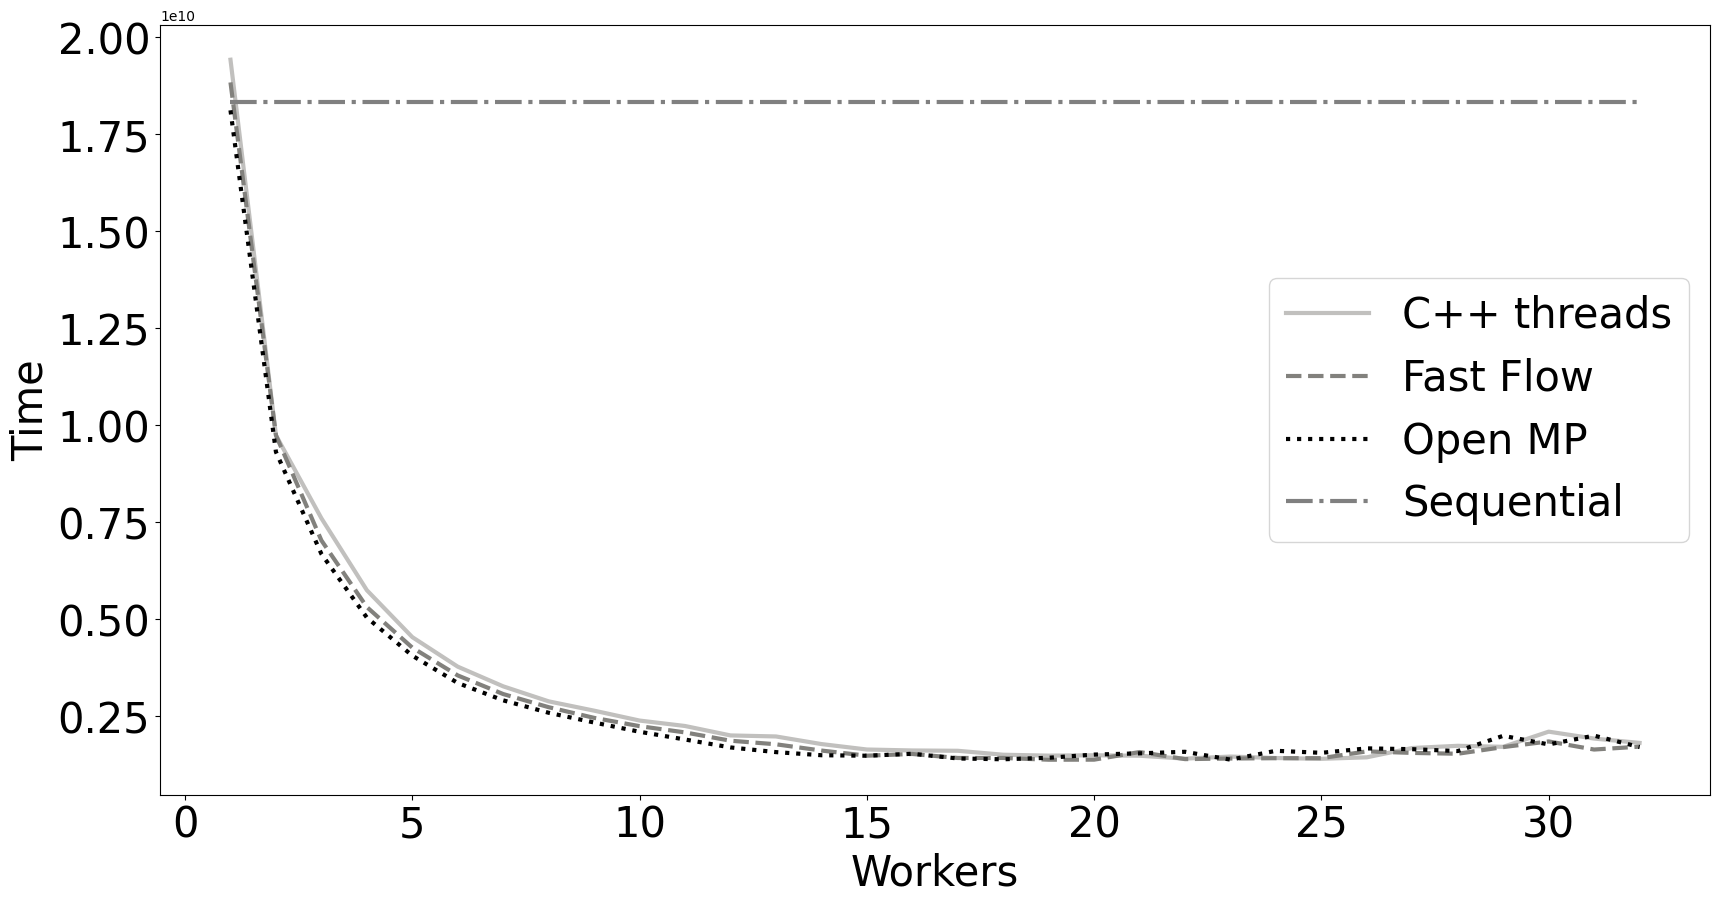
\includegraphics[width=13cm]{./images/time_vs_cores_10000}
		\caption{Time vs workers for matrix size 10000}
	\end{figure}

	\begin{figure}[H]
		\centering
		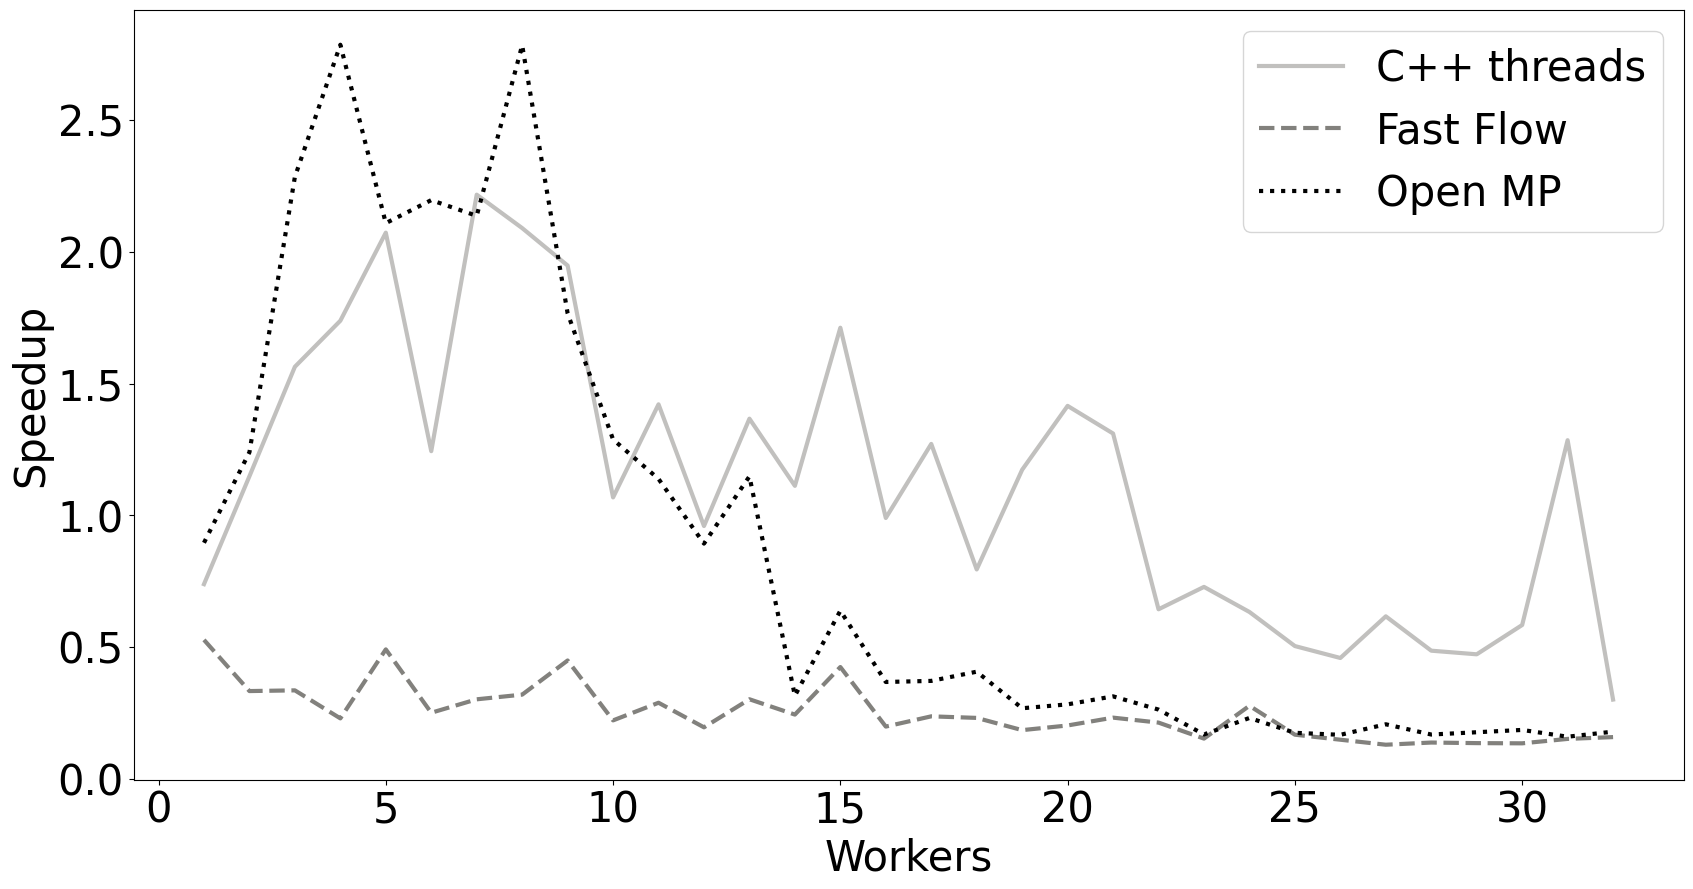
\includegraphics[width=13cm]{./images/speedup_vs_cores_1000}
		\caption{Speedup vs workers for matrix size 1000}
	\end{figure}

	\begin{figure}[H]
		\centering
		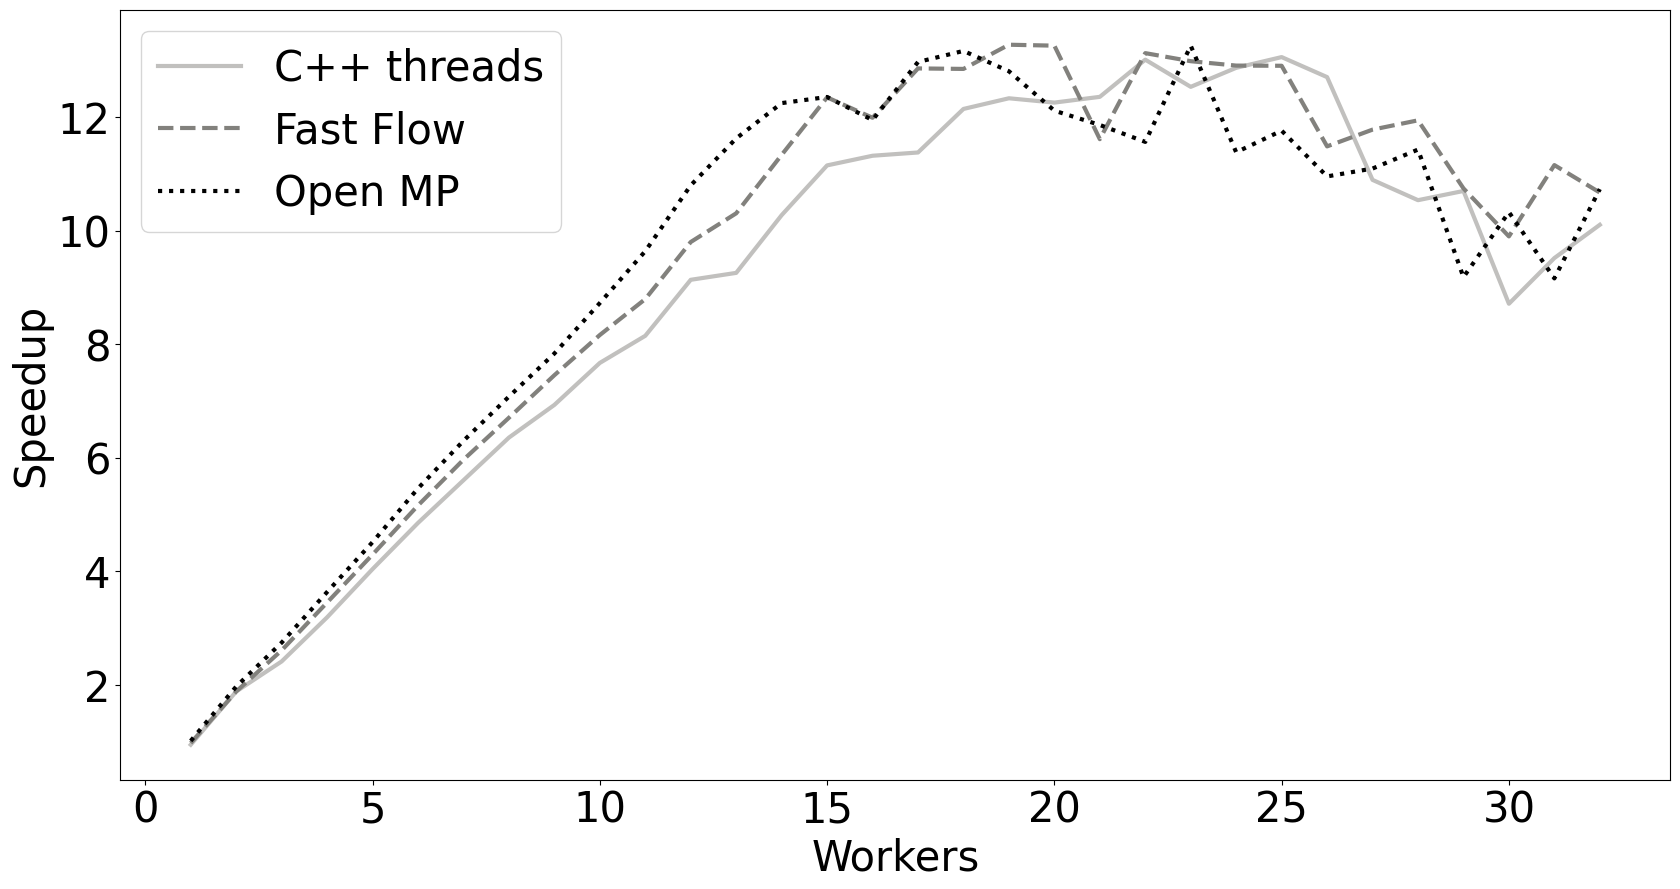
\includegraphics[width=13cm]{./images/speedup_vs_cores_10000}
		\caption{Speedup vs workers for matrix size 10000}
	\end{figure}

	\begin{figure}[H]
		\centering
		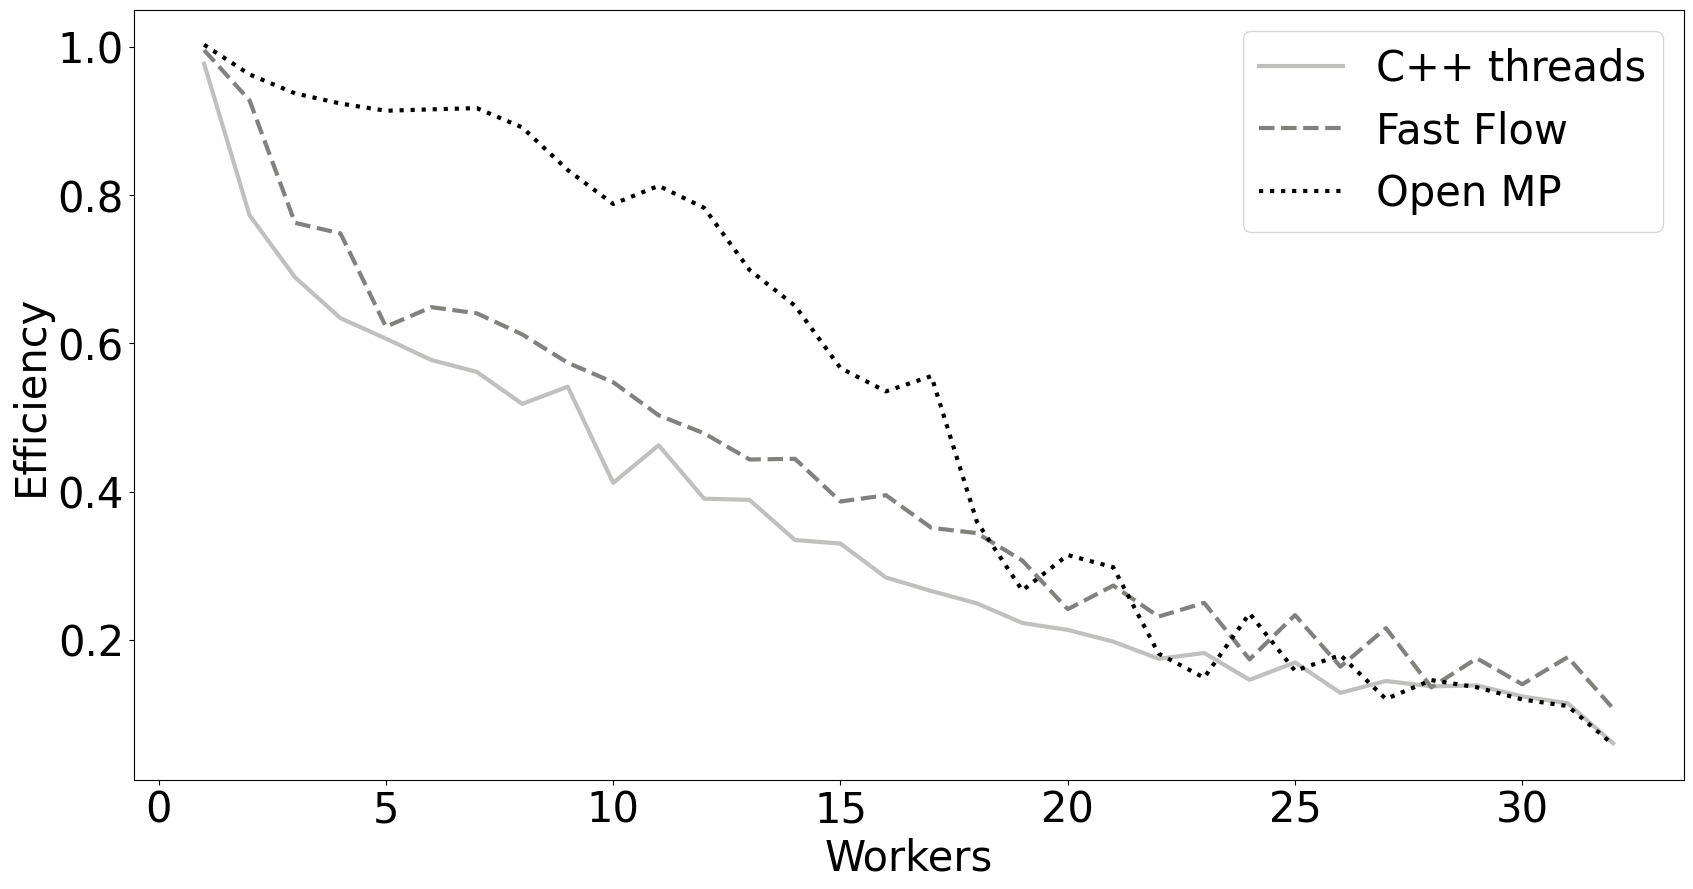
\includegraphics[width=13cm]{./images/efficiency_vs_cores_1000}
		\caption{Efficiency vs workers for matrix size 1000}
	\end{figure}

	\begin{figure}[H]
		\centering
		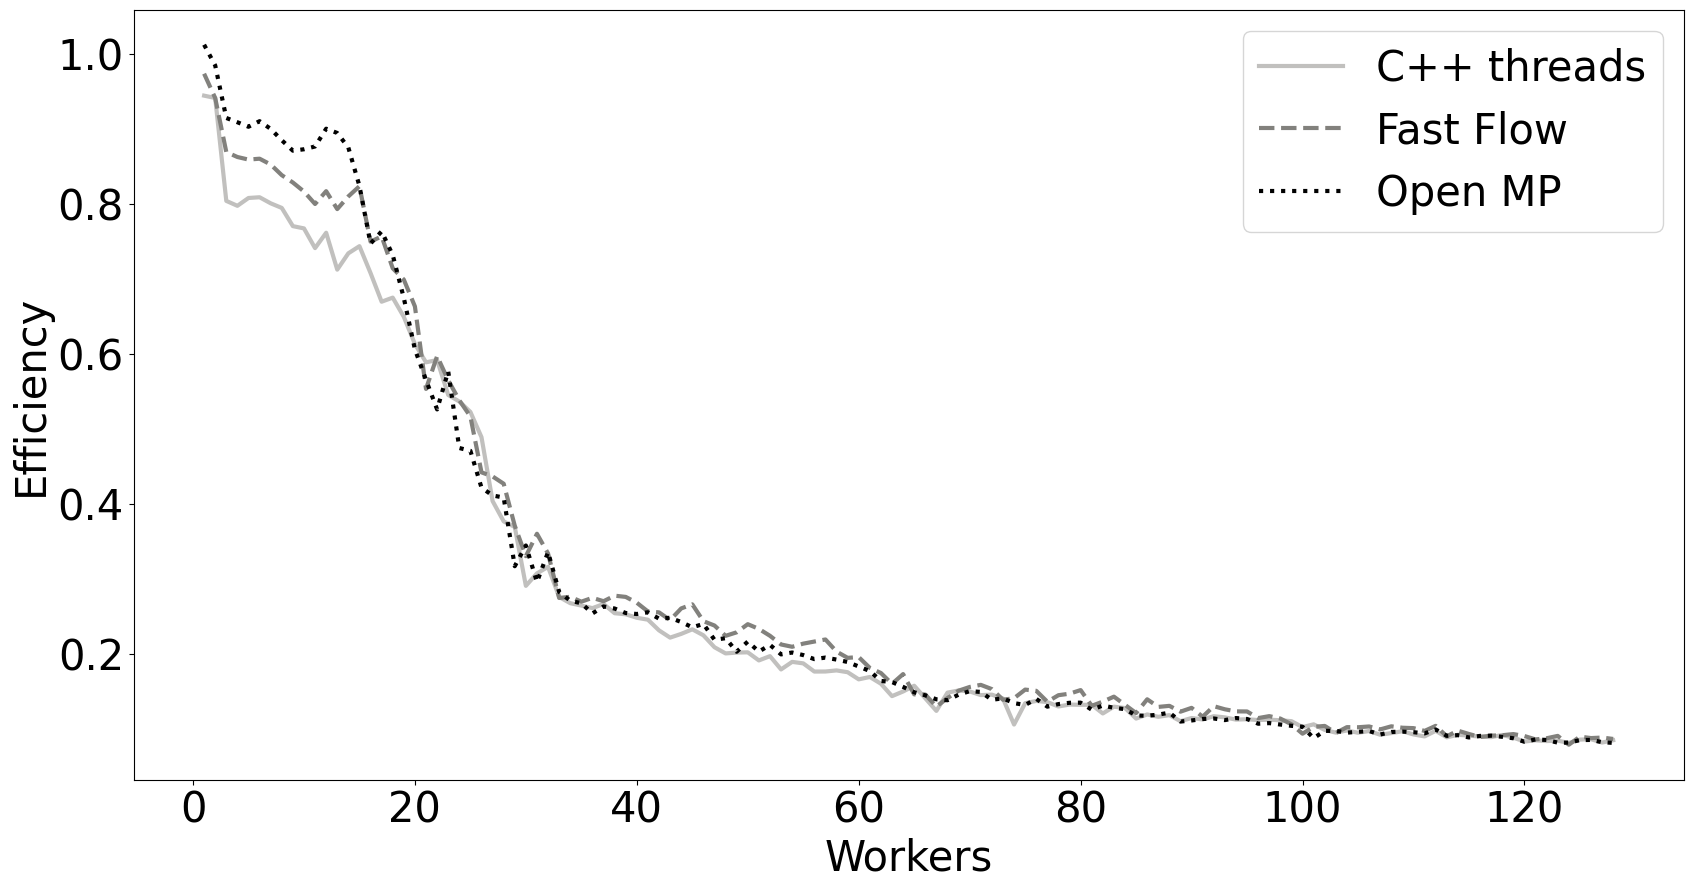
\includegraphics[width=13cm]{./images/efficiency_vs_cores_10000}
		\caption{Efficiency vs workers for matrix size 10000}
	\end{figure}

	\begin{figure}[H]
		\centering
		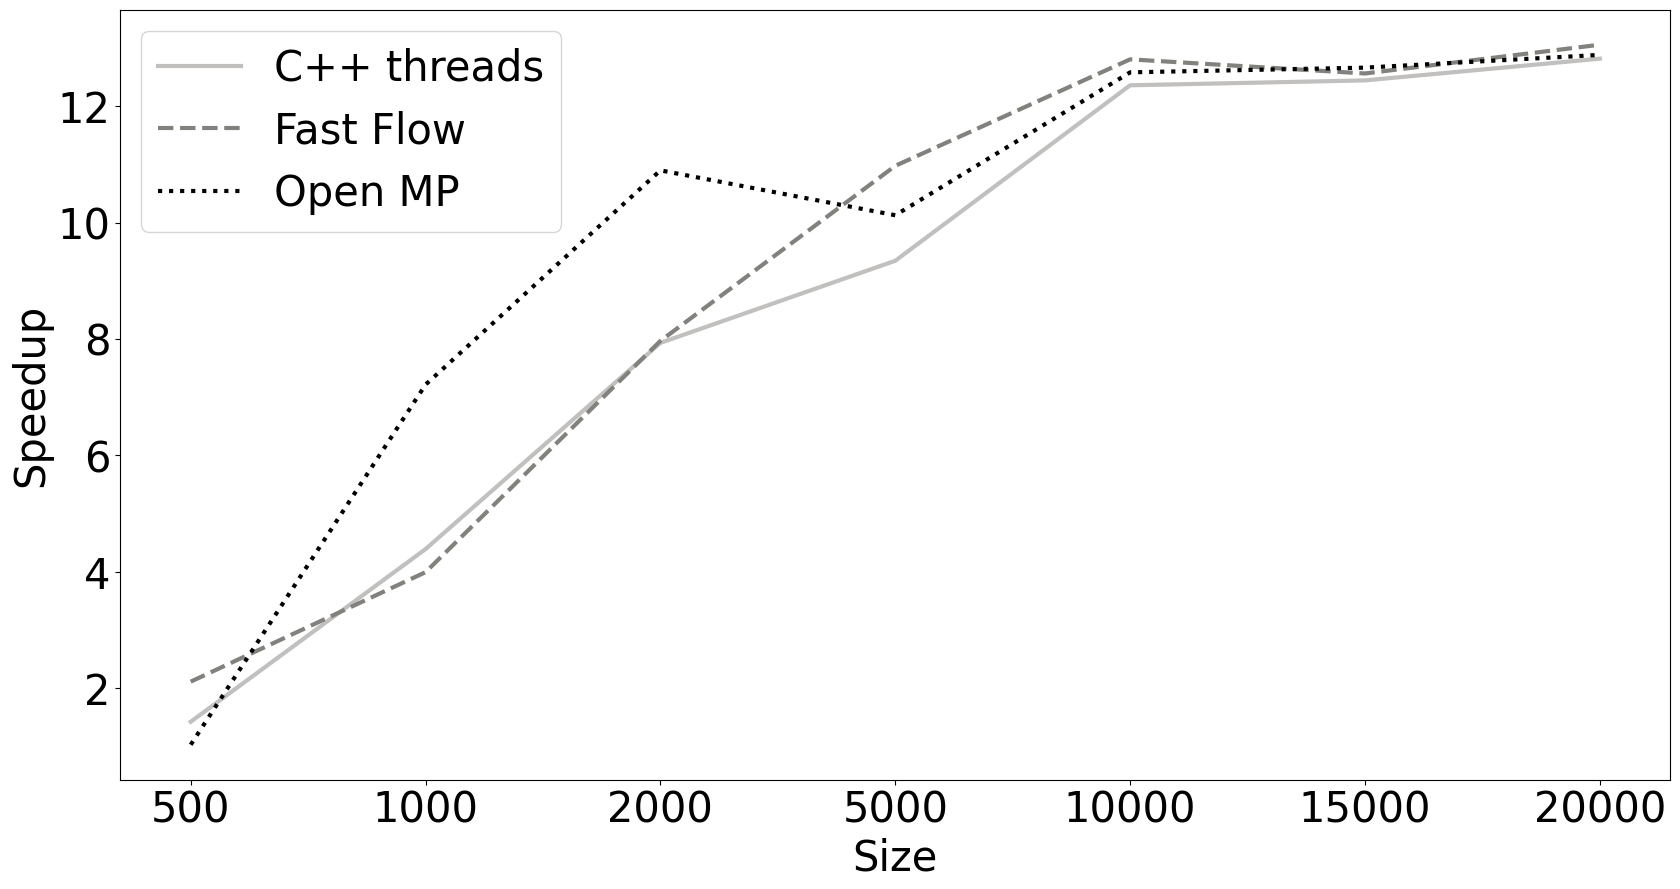
\includegraphics[width=13cm]{./images/speedup_vs_size}
		\caption{Speedup vs matrix size with 32 workers}
	\end{figure}

	\begin{figure}[H]
		\centering
		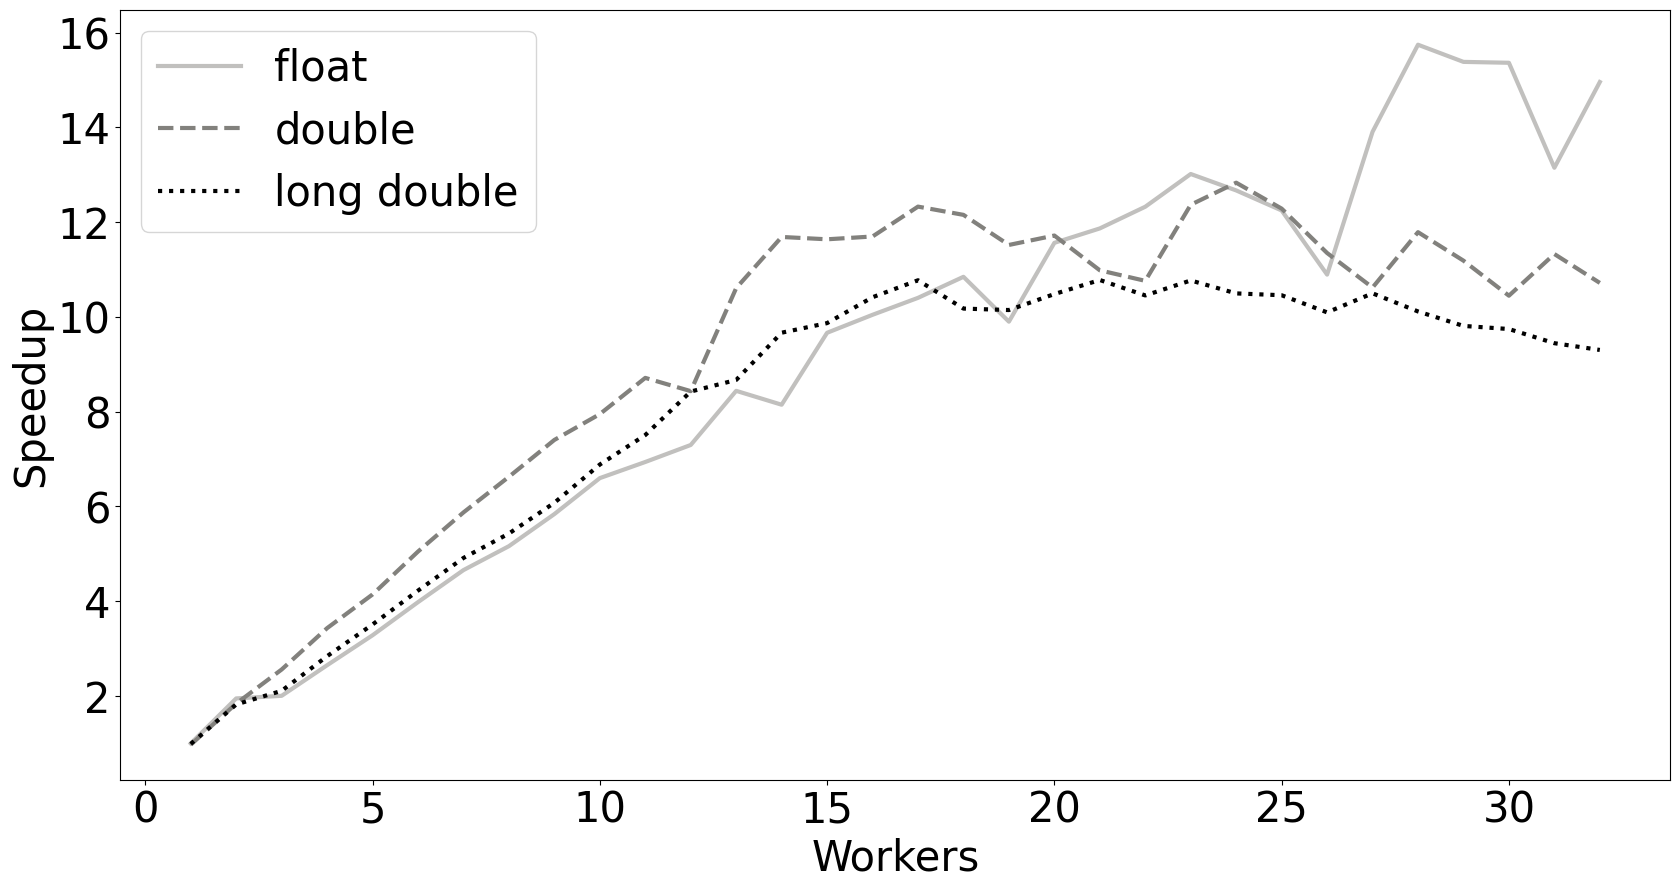
\includegraphics[width=13cm]{./images/data_types_speedup}
		\caption{Data types comparison}
	\end{figure}


	\section{Conclusions}
	The first thing that we notice from the experiments is that the performances are much better in the experiment where the matrix size is larger. When $n = 1000$ the maximum speedup (which is less then 8) around 10-20 workers, and then it starts to decrease. While in the case where $n = 10000$ we reach the maximum speedup again with more or less 10-20 workers, but then it remains stable around 8-10 even with an higher number of workers. Consequentially also the efficiency decrease slower when $n$ is large. This is also confirmed by figure \ref{fig:scaling}, that shows how the speedup increases while the matrix size increases. Probably executing test on larger matrices would bring a even better speedup, but the remote machine stopped the execution of the program when I tried with larger matrix sizes. Probably the better performances with larger sizes of the matrices are due to the fact, that increasing the size cause the grain of the computation of each worker to be coarser, and so the overhead has a reduced impact on the performances.\\
	In the case of $n = 1000$ we can se that with less than 20 workers, the OpenMP implementation is by far the better one, then as the number of threads increases the performances of the three versions are more or less the same, with FastFlow which tends to do slightly better. For $n = 10000$ we can se that the performances of the implementations are almost identical, even in this case at the beginning OpenMP tends to do slightly better, and FastFlow does a little bit better when the number of threads gets high.\\
	
	
\end{document}